\section{Analysis}
In this section, the use cases from the requirements section will be analysed
to provide the foundation for the design phase.

\subsection{Use Case analysis}
The first thing to do is to analyse the detailed use cases. This is done to find
the potential class candidates and to make an initial analyses class diagram.

\subsubsection{Class Candidates}
In order to find potential class candidates, every noun of the detailed Use
Cases are found. These are potential candidates and they are sorted to avoid
duplicates. Some of the candidates are note elaborate enough and will not be
turned into classes. Naturally, every potential class for the entire system will
not be found, as this only reflects use cases. A potential class candidate such
as MES (where Start and Stop functionality would otherwise be implemented) will
not be reduced to a single class and is therefore not added to the list of class
candidates.\\

The final list of classes, as well as a description of them, can be seen in
Table \ref{table:class_candidates}.

\begin{table}[ht]
    \captionof{table}{Potential class candidates}
    \begin{tabularx}{\textwidth}{|>{\RaggedRight}p{4cm}|>{\RaggedRight}p{6cm}|>{\RaggedRight}X|}
    \hline
    \textbf{Class Candidate} & \textbf{Attributes}                                                                                                     & \textbf{Definition}                                                                    \\ \hline
    Batch                    & Id, type, productAmount (total, defect, acceptable), amount (time), state (current, history), OEE, productionSpeed, & A batch refers to a specific batch of products the brewery has made                    \\ \hline
    Product                  & Id, type, ingredients                                                                                                  & Product refers to the different options of beer to be produced                         \\ \hline
    \end{tabularx}
    \label{table:class_candidates}
    \end{table}

\subsubsection{UML Analysis Diagram}
The UML analysis class diagram, seen in Figure \ref{figure:analysis_diagram},
can be generated based on the verb/noun analysis in the previous section. This
diagram shows the classes and attributes found in the requirements from the
project description.

\begin{figure}[ht]
	\centering 
	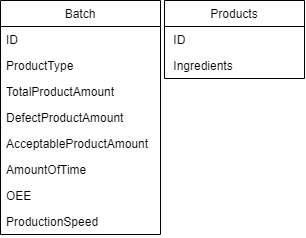
\includegraphics[scale=0.6]{images/diagrams/class_diagram.png}
	\caption{UML Analysis class diagram}
	\label{figure:analysis_diagram} 
\end{figure}

\subsection{Use Case Realisation}
To realise the scenarios in the use cases, use case realisation is used. In the
realisation it can be described how a scenario in the system should be designed.
The first step is to make operation contracts.

\subsubsection{Operation Contracts}
An operation contract describes the responsibility of an operation in the system.
These operations are found by making system sequence diagrams that display the
system as a 'black box', where the internal system events are not shown, but
only the external. This means that the diagram displays how actors generate
system events and what the system output is. Furthermore, the diagram functions
as a timeline for the system events. \\

The contract focuses on what the operation can change, and not how it is changed. 
It is also used to describes the state of the system before and after the 
operation is called. In Table \ref{table:Operation_Contracts_start} the
operation contract for the start operation can be seen.

\begin{table}[H]
    \captionof{table}{Operation Contracts Start} 
    \begin{tabularx}{\textwidth}{|>{\RaggedRight}p{3.7cm}|>{\RaggedRight}X|}
        \hline
        \multicolumn{2}{|c|}{\textbf{Start}}\\
        \hline
        \textbf{System operation} & Start\\
        \hline
        \textbf{Cross References} & Use case: Start machine, see Table \ref{table:usecase_start} \\
        \hline
        \textbf{Responsibility} & Starting the beer machine if the pre-conditions 
        is met. If the preconditions are not met, the beer machine will not
        start \\
        \hline
        \textbf{Output} & The beer machine started the production\\
        \hline
        \textbf{Pre-conditions} & The beer production machine needs to be in
        ready mode, that is, not producing beer and the necessary resources
        needs to be available. \\
        \hline
        \textbf{Post-conditions} & The beer machine started brewing\\
        \hline
    \end{tabularx}
    \label{table:Operation_Contracts_start}
\end{table}

\subsubsection{Operation Sequence Diagrams}
From the operation contracts, the operation sequence diagram can be made. The
operation sequence diagram displays the system as a 'white box', where both the
internal and external system events are described, as seen in Figure
\ref{figure:sequence_diagram}.

\begin{figure}[H]
\centering 
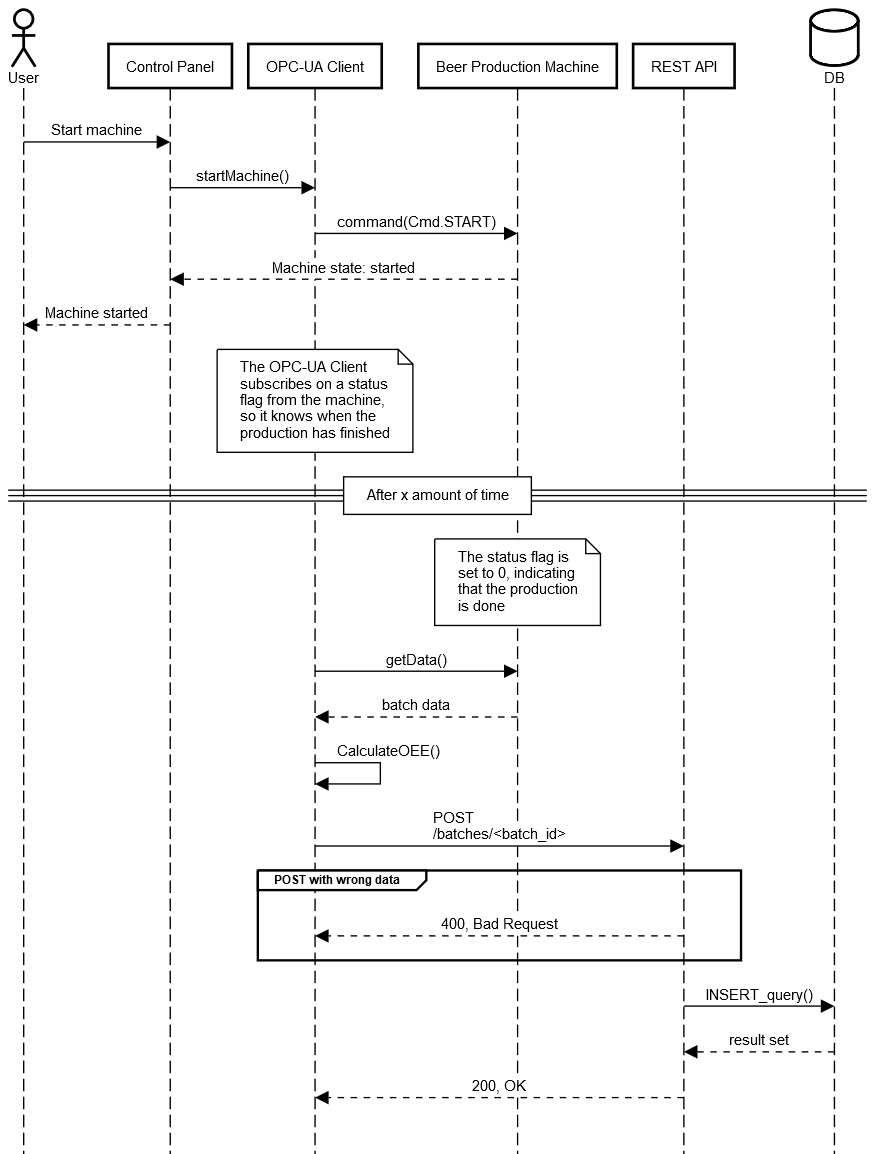
\includegraphics[width=1\linewidth]{images/sequence_operation/start.png}
\caption{Sequence diagram: start}
\label{figure:sequence_diagram} 
\end{figure}

This sequence diagram is used to identify system functions, as the events shown
in the diagram are the functions needed to complete the use case. In this
specific use case, the actor, the user, wants to start the beer production.
The user interacts with the dashboard by pressing the start button,
which then sends a command to the OPC-UA client via the API. The OPC-UA client
interprets the command as a 'start machine' command, which triggers an event in
the OPC-UA client to send a command to the beer production machine. The beer
production machine interprets the command as a start command, which then turns
on the machine. As a response to the user, to batch id is set on the dashboard.\\

When the beer production is running, the OPC-UA client sends all relevant
data from the beer production machine to the API. The API then send the data to
the dashboard, to show live production data. The data is also used to calculate
the optimal production speed, estimate the error function, and calculate the OEE.
These calculations are used to optimise the beer production. The calculated data
and the data collected from the machine is then stored in a database. This
happens through a REST API which acts as a translator between the different 
subsystems within the MES.

\subsubsection{Updated UML Class Diagram}
The updated UML class diagram seen in Figure 
\ref{figure:updated_UML_class_diagram} (see Appendix \ref{app:uml} for a larger
figure) illustrates the current system idea based on the analysis of the system.
Although this diagram only shows the OPC-UA client, it still gives a good idea
of how this part of the system is going to be, once implemented.

\begin{figure}[ht]
\centering 
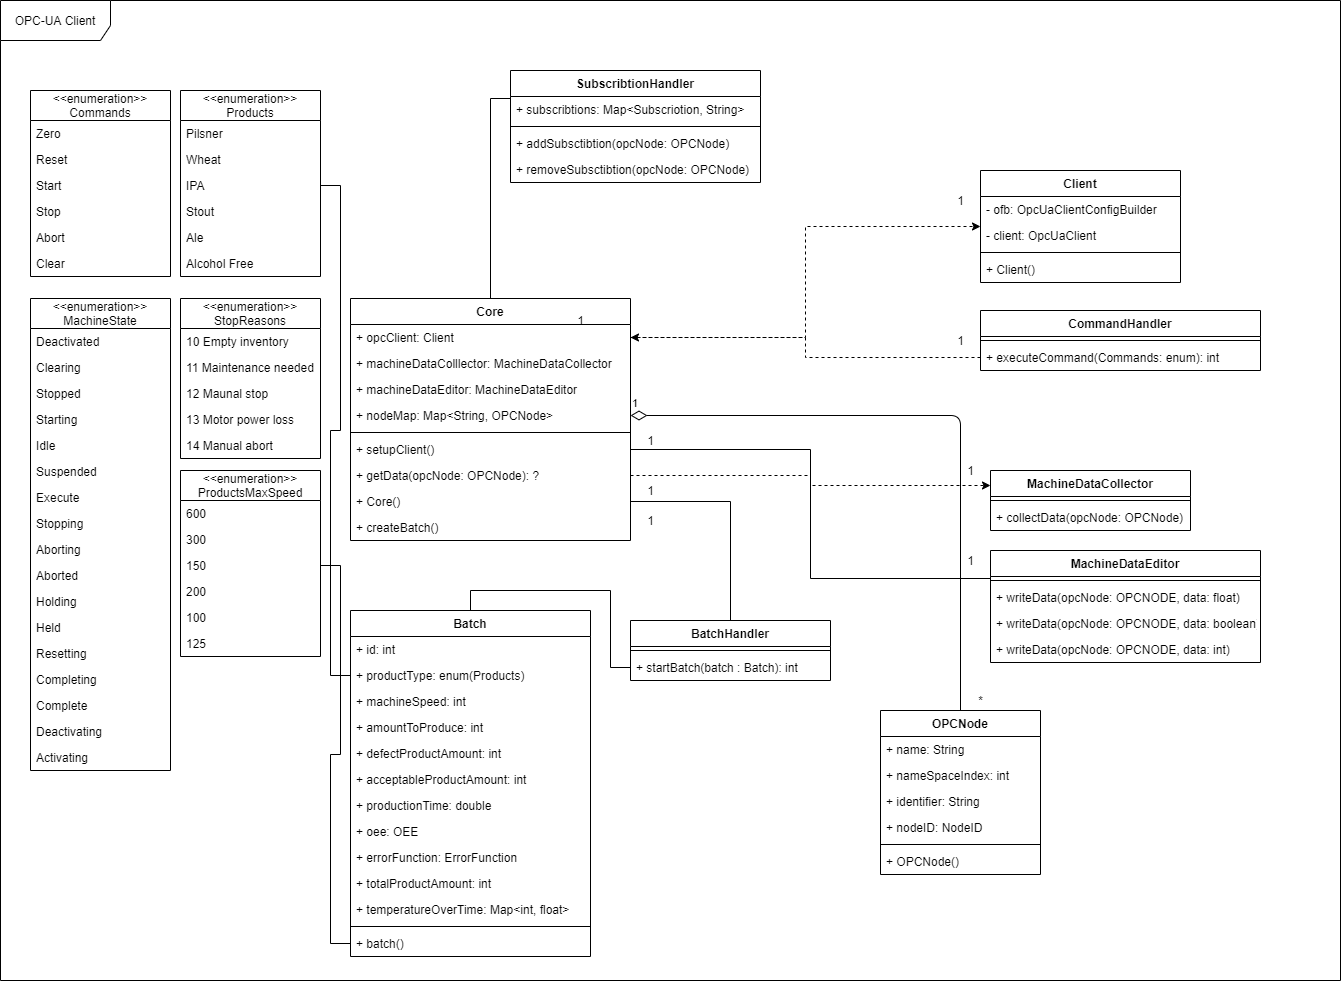
\includegraphics[width=1\textwidth]{images/diagrams/updated_UML_Class_Diagram.drawio.png}
\caption{Updated UML Class Diagram}
\label{figure:updated_UML_class_diagram} 
\end{figure}

By using the diagram in the implementation phase, the group has a good starting 
point to expand on. The classes in the UML class diagram have a chance of not 
being implemented if the group finds them unuseful or changed to adhere to the 
program. 
